\section{Kombinierte Regelung}
\subsection{Portierung des Balance-PID (Zander)}

Jonah Zanders Bachelorarbeit (2023) implementiert eine dreistufige Kaskadenregelung für ein selbstbalancierendes Fahrrad, die als Grundlage 
für die in dieser Arbeit entwickelte Simulationsregelung dient \cite{zander2023}. Die Hardware-Architektur umfasst einen BNO055-IMU-Sensor 
zur Neigungsmessung, einen BeagleBone-Black-Einplatinencomputer als Steuerungseinheit sowie separate Motorcontroller für Lenkung und Antrieb. 
Die Regelungsarchitektur gliedert sich in drei hierarchische Ebenen: eine primäre Balance-PID-Regelung (Angle-to-Steering), eine sekundäre 
Lenkpositionsregelung und eine vereinfachte Geschwindigkeitssteuerung.

\textbf{Primäre Balance-Regelung:} Das Kernstück von Zanders Implementierung bildet ein PID-Regler, der die Rollwinkelabweichung in einen 
Lenkwinkel-Sollwert umsetzt. Listing~\ref{lst:zander_pid_params} zeigt die von Zander gewählten PID-Parameter, die sich durch hohe 
proportionale (\(K_p = 10{,}0\)) und differentielle Verstärkungen (\(K_d = 2{,}2\)) bei deaktiviertem Integralanteil (\(K_i = 0{,}0\)) 
auszeichnen. Diese Parametrierung gewährleistet eine schnelle Reaktion auf Neigungsänderungen ohne die Gefahr des Aufschaukelns durch 
Drift-Integration.

\begin{lstlisting}[style=wbt_c,caption={PID-Parameter in Zanders Hardware-Implementierung},label={lst:zander_pid_params}]
//PID Angle to Steering
#define ANGLE_PID_KP                    10.0f
#define ANGLE_PID_KI                    0.0f
#define ANGLE_PID_KD                    2.2f 
#define ANGLE_PID_OUTPUT_MIN            -150.0f
#define ANGLE_PID_OUTPUT_MAX            150.0f
#define ANGLE_PID_INTEGRAL_MIN          -60.0f
#define ANGLE_PID_INTEGRAL_MAX          60.0f
\end{lstlisting}

Die PID-Berechnung in Zanders System implementiert eine zeitbasierte Integration und Differentiation mit Historien-Pufferung zur 
Rauschunterdrückung. Der Differentialterm wird über mehrere Zeitschritte gemittelt, um hochfrequente Störungen zu dämpfen, 
während der Integralterm durch Anti-Windup-Mechanismen begrenzt wird.

\textbf{Sekundäre Lenkpositionsregelung:} Die zweite Regelebene steuert den physischen Lenkmotor über einen MD49-Controller an, 
um den von der Balance-PID vorgegebenen Sollwinkel zu erreichen. Aufgrund der mechanischen Eigenschaften des Lenkantriebs 
(Reibung, Trägheit, Totzeit) sind hier deutlich höhere Verstärkungen erforderlich:

\begin{lstlisting}[style=wbt_c,caption={Lenkpositions-PID-Parameter in Zanders System},label={lst:zander_steering_pid}]
//PID Steering PID
#define MD49_PID_KP                     850.0f
#define MD49_PID_KI                     300.0f
#define MD49_PID_KD                     30.0f
#define MD49_PID_OUTPUT_MIN             -100000.0f
#define MD49_PID_OUTPUT_MAX             100000.0f
\end{lstlisting}

\textbf{Echtzeit-Threading-Architektur:} Zanders Implementierung nutzt eine multi-threaded Architektur mit unterschiedlichen 
Abtastraten: IMU-Datenerfassung mit 200\,Hz, Lenkpositionsregelung mit 1000\,Hz und Geschwindigkeitsregelung mit niedrigerer 
Frequenz. Watchdog-Mechanismen überwachen die Thread-Ausführung und gewährleisten die Systemstabilität bei Hardwareausfällen.

\textbf{Adaptierung für die Webots-Simulation:} Die Portierung von Zanders Balance-Regelung in die Webots-Simulationsumgebung 
erforderte eine systematische Vereinfachung der Hardware-spezifischen Komplexitäten bei Beibehaltung der regelungstechnischen 
Kernprinzipien. Die wesentlichen Unterschiede zwischen Hardware- und Simulationsimplementierung zeigt Tabelle~\ref{tab:zander_comparison}.

\begin{table}[H]
\centering
\caption{Vergleich zwischen Zanders Hardware-Implementierung und Webots-Simulation}
\label{tab:zander_comparison}
\begin{tabular}{|l|l|l|}
\hline
\textbf{Aspekt} & \textbf{Zander (Hardware)} & \textbf{Webots-Simulation} \\
\hline
Sensorik & BNO055 IMU, Rauschen & Idealer Rollwinkelsensor \\
Threading & Multi-threaded (200/1000 Hz) & Synchrone Hauptschleife \\
Lenkpositionsregelung & Separater MD49-PID & Direkter Motoranschluss \\
PID-Parameter & $K_p=10, K_i=0, K_d=2.2$ & Identische Werte \\
Ausgangsbegrenzung & $\pm 150$ (Hardware-Einheiten) & $\pm 0.3$ rad \\
\hline
\end{tabular}
\end{table}

Die Webots-Implementierung vereinfacht die Architektur erheblich durch Elimination der sekundären Lenkpositionsregelung. 
Listing~\ref{lst:webots_balance_pid} zeigt die zentrale Balance-Regelschleife, die direkt den Lenkwinkel setzt:

\begin{lstlisting}[style=wbt_c,caption={Vereinfachte Balance-PID-Implementierung in Webots},label={lst:webots_balance_pid}]
// 1. Roll-Winkel messen (idealisiert, ohne Rauschen)
float roll_angle = get_roll_rad_raw();

// 2. PID-Regelung: Roll-Winkel -> Lenkwinkel  
if (control_enabled) {
    steering_output = -pid_compute(&angle_pid, 0.0, roll_angle, current_time);
}

// 3. Lenkwinkel begrenzen
if (steering_output > config.mechanical_limits.max_handlebar_angle) 
    steering_output = config.mechanical_limits.max_handlebar_angle;
else if (steering_output < -config.mechanical_limits.max_handlebar_angle)
    steering_output = -config.mechanical_limits.max_handlebar_angle;

// 4. Direkter Motoranschluss (keine sekundaere Regelung)
wb_motor_set_position(handlebars_motor, -final_steer);
\end{lstlisting}

Der PID-Algorithmus selbst wurde von Zanders Implementierung adaptiert, jedoch mit verbesserter numerischer Stabilität. 
Während Zanders Code eine komplexe Historien-Verwaltung mit zirkulären Puffern verwendet, nutzt die Webots-Version eine 
vereinfachte Zeitberechnung basierend auf dem deterministischen Simulationszeitschritt:

\begin{lstlisting}[style=wbt_c,caption={Vereinfachte PID-Berechnung in der Webots-Implementierung},label={lst:webots_pid_compute}]
// I-Term (Integral) - vereinfachte Zeitberechnung
int prev_index = (pid->history_counter + HISTORY_LEN - 1) % HISTORY_LEN;
float dt = (pid->time_history[pid->history_counter] - 
           pid->time_history[prev_index]) / 1000000.0; // Mikrosekunden -> Sekunden

if (dt > 0.0 && dt < 1.0) {  // Plausibilitaetspruefung
    pid->integral_term += pid->Ki * error * dt; 
}

// D-Term mit gleitendem Durchschnitt (wie bei Zander)
float current_derivative = (error - pid->error_history[prev_index]) / dt;
pid->derivative_history[pid->history_counter] = current_derivative;

float derivative_sum = 0.0;
for (int i = 0; i < HISTORY_LEN; i++) {
    derivative_sum += pid->derivative_history[i];
}
pid->derivative_term = pid->Kd * (derivative_sum / HISTORY_LEN);
\end{lstlisting}

Die erfolgreiche Übertragung von Zanders Regelungskonzept in die Simulation bestätigt 
die Robustheit des gewählten PID-Ansatzes. Die identischen Parameter (\(K_p = 10\), \(K_i = 0\), \(K_d = 2{,}2\)) erzielen 
auch in der idealisierten Webots-Umgebung stabile Balance-Regelung. Der Verzicht auf den Integralanteil erweist sich als 
vorteilhaft, da er Drift-bedingte Instabilitäten vermeidet, was ein Aspekt, der sowohl in der Hardware- als auch in der 
Simulationsumgebung relevant ist.

Die Portierung demonstriert, wie Hardware-spezifische Komplexitäten (Multi-Threading, Sensor-Rauschen, Aktor-Totzeiten) in 
einer Simulationsumgebung abstrahiert werden können, ohne die regelungstechnischen Kernprinzipien zu beeinträchtigen. 
Diese Vereinfachung schafft die Grundlage für die Integration zusätzlicher Regelungsebenen, insbesondere der vision-basierten 
Pfadführung, die in den folgenden Abschnitten behandelt wird.


  
\subsection{Portierung des Fahrtrichtungs-MPC (Giray)} \label{chap:MPC_KAPITEL}
Yasin Giray entwickelte in seiner Masterarbeit einen vision-basierten 
Fahrtrichtungsregler auf Basis von Model Predictive Control (MPC), 
um das selbstbalancierende Fahrrad autonom der Fahrspur folgen zu lassen \cite{vision_mpc_readme}. Dieser Regler modelliert die Fahrzeugdynamik mittels Einspurmodell 
und nutzt zwei Steuergrößen, die aktuelle Geschwindigkeit \(v\) und Lenkwinkel \(\phi\) als Eingaben für die Prädiktion. Der MPC berechnet 
also auf Grundlage von \(v\) und Lenkeinschlag die Fahrzeugbewegung voraus. Für den prädiktiven Regler wird ein 
Zustandsvektor \(x=[x, y, v, \text{yaw}]\) (Position, Geschwindigkeit, Gierwinkel) und ein Eingangsvektor \(u=[\text{accel}, \text{steer}]\) 
definiert. Giray wählte einen Zeithorizont von etwa 2~s und formulierte ein Optimierungsproblem, das die Abweichung von einer Soll-Trajektorie 
minimiert sowie Steuerungsaufwand und -änderungen übernimmt. Die Kostenfunktion des MPC addiert quadrierte Abweichungen der Zustände und Eingriffe über den Horizont sowie eine 
Endzustands-Strafe, z.\,B. \(J=\sum (x^T Q x + u^T R u + \Delta u^T R_d \Delta u) + x_{\text{final}}^T Q_f x_{\text{final}}\) \cite{vision_mpc_readme}. 
Neben den Kosten werden physikalische Nebenbedingungen wie maximaler Lenkwinkel, Lenkwinkelrate und Geschwindigkeit im Optimierungsproblem 
berücksichtigt, um realistische Lösungen zu gewährleisten.

Wesentliche Voraussetzung für den Fahrtrichtungs-MPC ist eine geeignete Referenztrajektorie der Straße. Giray implementierte hierfür eine 
Computer-Vision-Pipeline auf Basis von YOLOv8-Segmentierung, welche im Kamerabild die befahrbare Straße und deren Verlauf erkennt. Aus den 
segmentierten Bilddaten wird eine Reihe von Stützpunkten der Fahrbahn extrahiert. Anschließend 
wird mittels Spline-Interpolation eine glatte Kurve durch diese Punkte gelegt, die als Referenzkurve für den MPC dient. Er simuliert auf Basis des Einspurmodells die Fahrzeugbewegung und berechnet die optimalen 
Steuerbefehle, damit das Fahrrad der Kurve bestmöglich folgt. In Girays Umsetzung wird der Regler zyklisch mit ca. 10 Hz ausgeführt (Tickrate 100 ms). 
Pro Zyklus initialisiert der Controller den aktuellen Fahrzeugzustand (Position, Geschwindigkeit, Orientierung) und berechnet aus der ersten Sollkurve 
einen Vorhersagepfad. Die Optimierung liefert dann eine Stellgrößen-Sequenz für Beschleunigung und Lenkwinkel. 
Tatsächlich wird nur der erste Lenkwinkel-Impuls umgesetzt (Receding Horizon Control), welcher als neuer Lenkbefehl an das Fahrzeug geht. 
Im nächsten Zyklus wird der MPC erneut mit aktualisiertem Zustand und ggf. angepasster Referenz gestartet. Giray konnte in Simulationen zeigen, 
dass der MPC-Regler das Fahrrad effektiv der vorgegebenen Spur folgen lässt. Die geplante Spline-Trajektorie und die vom MPC gefahrene 
Ist-Trajektorie in seiner Arbeit, stimmen dabei eng überein, was die Güte der prädiktiven Regelung belegt.


\textbf{Adaptierung für Webots-Simulation:} Die Portierung von Girays MPC-Konzept in die Webots-Umgebung erforderte eine systematische 
Anpassung an die spezifischen Anforderungen der Simulation und Integration mit dem vorhandenen Balance-Controller. Tabelle~\ref{tab:giray_comparison} 
zeigt die wesentlichen Unterschiede zwischen Girays theoretischem Ansatz und der Webots-Implementierung.

\begin{table}[H]
\centering
\caption{Vergleich zwischen Girays MPC-Konzept und Webots-Implementierung}
\label{tab:giray_comparison}
\begin{tabular}{|l|l|l|}
\hline
\textbf{Aspekt} & \textbf{Giray (Theorie)} & \textbf{Webots-Implementierung} \\
\hline
Prädiktionshorizont & N=20 (2\,s - 10\,Hz) & T=3 (0.3\,s - 20\,Hz) \\
Referenzgenerierung & Spline-Interpolation & Vereinfachte Korrekturtrajectorie \\
Zustandsvektor & $[x, y, v, \psi]^T$ & $[x, y, v, yaw]^T$ (identisch) \\
Eingangsvektor & $[a, \delta]^T$ & $[accel, steer]^T$ (identisch) \\
Regelfrequenz & 10\,Hz & 20\,Hz \\
Optimierer & CVXPY (theoretisch) & CVXPY (praktisch) \\
Integration & Standalone & Gekoppelt mit Balance-PID \\
\hline
\end{tabular}
\end{table}

Die Webots-Implementierung vereinfacht Girays Ansatz erheblich durch Reduzierung des Prädiktionshorizonts auf 3 Zeitschritte 
(\(\approx 0{,}3\,\mathrm{s}\)). Diese Entscheidung wurde aus Echtzeitgründen getroffen, da die Integration mit dem Balance-Controller 
eine höhere Regelfrequenz (20\,Hz) erfordert. Listing~\ref{lst:webots_mpc_init} zeigt die Initialisierung des MPC-Controllers 
mit den angepassten Parametern:

\begin{lstlisting}[style=python,caption={MPC-Controller Initialisierung in der Webots-Implementierung},label={lst:webots_mpc_init}]
def __init__(self):
    # MPC-Parameter (reduziert gegenueber Giray)
    self.NX = 4  # Zustandsvektor: [x, y, v, yaw]
    self.NU = 2  # Eingaenge: [accel, steer]
    self.T = 3   # Praediktionshorizont (reduziert fuer Echtzeitfaehigkeit)
    
    # Kostenmatrizen (aehnlich Girays Formulierung)
    self.R = np.diag([0.01, 0.01])      # Eingangskostenmatrix
    self.Rd = np.diag([0.01, 1.0])      # Eingangsdifferenzkostenmatrix
    self.Q = np.diag([1.0, 1.0, 0.5, 0.5])  # Zustandskostenmatrix
    self.Qf = self.Q                    # Terminale Kostenmatrix
    
    # Fahrzeugparameter (Bicycle-Modell)
    self.WB = 1.2  # Radstand [m] (Fahrrad)
    self.DT = 0.1  # Zeitschritt [s]
    
    # Physikalische Begrenzungen
    self.MAX_STEER = math.radians(30.0)  # Maximaler Lenkwinkel
    self.MAX_DSTEER = math.radians(20.0) # Maximale Lenkwinkelrate
    self.MAX_SPEED = 8.0                 # Maximale Geschwindigkeit
    self.MIN_SPEED = 0.5                 # Minimale Geschwindigkeit
\end{lstlisting}

Anstelle von Girays komplexer Spline-Interpolation aus Bildpunkten verwendet die Webots-Implementierung eine vereinfachte 
Referenzgenerierung basierend auf dem aktuellen Vision-Fehler. Die Referenztrajektorie wird aus dem lateralen Spurabweichungsfehler 
abgeleitet, indem ein Ziel-Gierwinkel berechnet und über den kurzen Horizont interpoliert wird.

\textbf{MPC-Optimierungsalgorithmus:} Die Webots-Implementierung folgt Girays theoretischer Formulierung bei der Lösung des 
Optimierungsproblems. Listing~\ref{lst:webots_mpc_solver} zeigt den Kern des MPC-Algorithmus:

\begin{lstlisting}[style=python,caption={MPC-Optimierungsalgorithmus in der Webots-Implementierung},label={lst:webots_mpc_solver}]
def linear_mpc_control(self, xref, xbar, x0):
    """Loest MPC-Optimierungsproblem"""
    try:
        x = cvxpy.Variable((self.NX, self.T + 1))
        u = cvxpy.Variable((self.NU, self.T))
        
        cost = 0.0
        constraints = []
        
        for t in range(self.T):
            cost += cvxpy.quad_form(u[:, t], self.R)
            
            if t != 0:
                cost += cvxpy.quad_form(xref[:, t] - x[:, t], self.Q)
            
            A, B, C = self.get_linear_model_matrix(
                xbar[2, t], xbar[3, t], 0.0)  # Linearisierung um Referenz
            constraints += [x[:, t + 1] == A @ x[:, t] + B @ u[:, t] + C]
            
            if t < (self.T - 1):
                cost += cvxpy.quad_form(u[:, t + 1] - u[:, t], self.Rd)
                constraints += [cvxpy.abs(u[1, t + 1] - u[1, t]) <= self.MAX_DSTEER * self.DT]
        
        cost += cvxpy.quad_form(xref[:, self.T] - x[:, self.T], self.Qf)
        
        # Randbedingungen
        constraints += [x[:, 0] == x0]
        constraints += [x[2, :] <= self.MAX_SPEED]
        constraints += [x[2, :] >= self.MIN_SPEED]
        constraints += [cvxpy.abs(u[0, :]) <= self.MAX_ACCEL]
        constraints += [cvxpy.abs(u[1, :]) <= self.MAX_STEER]
        
        # Problem loesen
        prob = cvxpy.Problem(cvxpy.Minimize(cost), constraints)
        prob.solve(verbose=False)
        
        if prob.status == cvxpy.OPTIMAL or prob.status == cvxpy.OPTIMAL_INACCURATE:
            u_opt = u.value
            if u_opt is not None:
                return u_opt[0, 0], u_opt[1, 0]  # Erste Kontrollaktion
        
        return self._simple_control_fallback(xref, x0)
        
    except Exception as e:
        return self._simple_control_fallback(xref, x0)
\end{lstlisting}

Die Implementierung folgt dem Standard-MPC-Schema mit quadratischen Kosten und linearen Constraints. Im Gegensatz zu Girays 
längerfristigem Horizont ermöglicht die Reduzierung auf 3 Zeitschritte eine Echtzeitausführung mit 20\,Hz.

\textbf{Integration mit Balance-Controller:} Ein wesentlicher Unterschied zu Girays Standalone-Ansatz liegt in der Integration mit 
dem bestehenden Balance-PID-Regler. Die Webots-Implementierung realisiert eine Kaskadenregelung, bei der der MPC-Controller die 
langfristige Spurführung übernimmt, während der Balance-PID die kurzfristige Stabilisierung gewährleistet. Die MPC-Ausgaben werden 
normalisiert und über IPC an den C-basierten Balance-Controller übertragen:

\begin{lstlisting}[style=python,caption={IPC-Übertragung der MPC-Kommandos an den Balance-Controller},label={lst:mpc_ipc}]
def send_vision_command(self, steer_cmd, speed_cmd):
    """Sendet erweiterte Vision-Command an Balance-Controller"""
    try:
        # Begrenzungen anwenden
        steer_cmd = max(-1.0, min(1.0, steer_cmd))
        speed_cmd = max(0.0, min(1.0, speed_cmd))
        
        # Erweiterte Struct-Format: 8 Felder
        # (steer_command, speed_command, valid, vision_error, 
        #  vision_p_term, vision_i_term, vision_d_term, mask_coverage)
        command_data = struct.pack('ffifffff', 
                                 steer_cmd, speed_cmd, 1,
                                 self.vision_error, self.mpc_controller.mpc_p_term, 
                                 self.mpc_controller.mpc_i_term, self.mpc_controller.mpc_d_term, 
                                 self.vision_mask_coverage)
        
        self.command_emitter.send(command_data)
        return True
    except Exception as e:
        return False
\end{lstlisting}

\textbf{Bewertung der Portierung:} Die Adaptation von Girays MPC-Konzept für die Webots-Simulation demonstriert sowohl die 
Übertragbarkeit theoretischer MPC-Ansätze als auch die Notwendigkeit praktischer Kompromisse.
Die vereinfachte Referenzgenerierung verzichtet auf Girays komplexe Spline-Interpolation, bietet jedoch ausreichende Genauigkeit 
für die Spurhaltung in der Simulation.

Die erfolgreiche Kopplung mit dem Balance-Controller zeigt, dass MPC-basierte Spurführung und PID-basierte Stabilisierung 
komplementäre Regelungsebenen darstellen können. Girays theoretischer Beitrag zur modellprädiktiven Fahrzeugführung findet 
somit praktische Anwendung in einem hybriden Regelungskonzept, das die Vorteile beider Ansätze kombiniert.

\newpage


\subsection{Strategien der Spurführung}

Die Vision-basierte Spurführung des selbstbalancierenden Fahrrads nutzt zwei unterschiedliche Erkennungsstrategien: 
eine YOLO-basierte Segmentierung als Hauptverfahren und eine robuste Fallback-Strategie für Ausfallsituationen. 
Beide Verfahren extrahieren aus dem Kamerabild einen lateralen Spurabweichungsfehler, der vom zuvor beschriebenen MPC 
in Lenkbefehle umgesetzt wird.

\subsubsection{YOLO-Segmentierung (YOLOv8)}

Die YOLO-Strategie nutzt ein vortrainiertes YOLOv8-Segmentierungsmodell zur robusten Erkennung der Fahrbahn. 
Das neuronale Netz identifiziert Straßenbereiche als Klasse \enquote{street\_main} und liefert sowohl Bounding Boxes 
als auch pixelgenaue Segmentierungsmasken, wie in Kapitel \ref{chap:yolo} beschrieben ist.
Das System sucht beim Start nach einer trainierten Gewichtsdatei (\texttt{best.pt}) 
und lädt das YOLOv8-Modell auf das verfügbare Rechengerät. Bei Nichtverfügbarkeit erfolgt automatischer Wechsel 
zur Fallback-Strategie:

\begin{lstlisting}[style=python,caption={YOLO-Modell Initialisierung},label={lst:yolo_init}]
  if YOLO_AVAILABLE:
    possible_paths = [
        "../balance_control_c/yolo_vision/runs/segment/train/weights/best.pt",
        "yolo_weights/best.pt",
        "best.pt"
    ]
    for path in possible_paths:
        if os.path.exists(path):
            try:
                device = "mps" if torch.backends.mps.is_available() else \
                         ("cuda" if torch.cuda.is_available() else "cpu")
                self.yolo_model = YOLO(path).to(device)
                print(f"[OK] YOLO-Modell geladen: {path} (Device: {device})")
                break
            except Exception as e:
                print(f"[WARN] Fehler beim Laden von {path}: {e}")
                continue
    if not self.yolo_model:
        print("[WARN] Kein YOLO-Modell gefunden - Fallback-Vision aktiviert")
        YOLO_AVAILABLE = False
\end{lstlisting}


Im Echtzeitbetrieb (20\,Hz) analysiert YOLO jedes Kamerabild und filtert Straßenobjekte 
(Klasse \enquote{street\_main}). Aus den Bounding Boxes aller erkannten Straßenbereiche wird der gemittelte Mittelpunkt berechnet. Die laterale 
Abweichung ergibt sich als normierte Differenz zwischen Straßenmittelpunkt und Bildmitte (\texttt{error} $\in [-0.5, +0.5]$):

\begin{figure}[H]
  \centering
  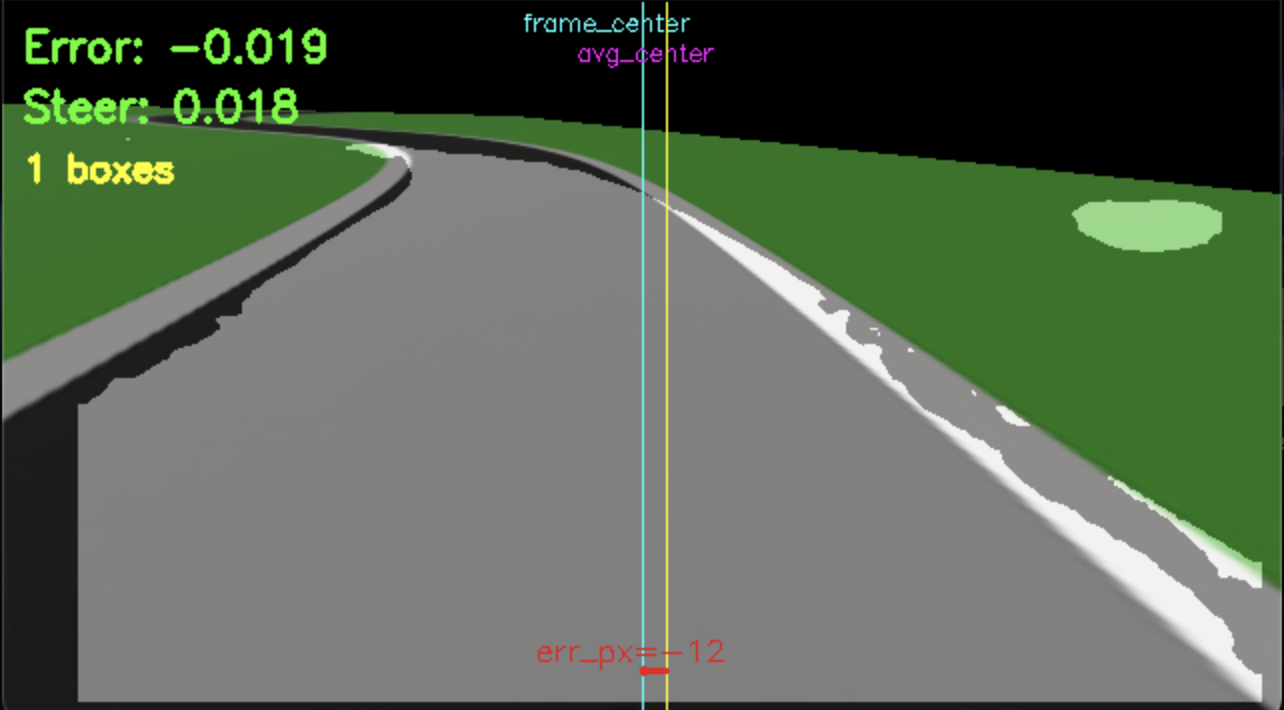
\includegraphics[width=0.8\textwidth]{figures/Yolo_Snapshot.png}
  \caption{YOLOv8-Segmentierung.}
  \label{fig:yolov8}
\end{figure}


\begin{lstlisting}[style=python,caption={YOLO-Fehlerberechnung},label={lst:yolo_error_calculation}]
  street_indices = [idx for idx, cls in enumerate(r.boxes.cls) if cls == 2]
  if street_indices:
      x_centers = []
      for idx in street_indices:
          xyxy = r.boxes.xyxy[idx]  # Koordinaten der Bounding Box
          x_center = float((xyxy[0] + xyxy[2]) / 2.0)
          x_centers.append(x_center)
      avg_x_center = sum(x_centers) / len(x_centers)
      frame_center = frame.shape[1] / 2
      error = (frame_center - avg_x_center) / frame.shape[1]  # Normiert
      self._store_valid_values(error, mask, self.vision_mask_coverage)
      return error, mask
\end{lstlisting}

Das System implementiert eine Ausfallüberbrückung durch Zwischenspeicherung 
der letzten gültigen Fehlerwerte. Bei Detektionsaussetzern wird der gespeicherte Fehler mit Decay-Faktor schrittweise 
abgeschwächt, bis er nach definierten Ausbleib-Zyklen auf Null fällt. Dies verhindert abrupte Lenkbewegungen bei 
temporären Erkennungsverlusten.




\textbf{Limitierungen:} Die YOLO-Strategie erfordert ein geeignetes vortrainiertes Modell und ausreichende 
Rechenleistung. Bei Abweichungen von den Trainingsdaten können Fehlerkennungen auftreten. Diese Fehlererkennungen 
werden in Kapitel \ref{chap:teststrecken} beschrieben. 



\subsubsection{Fallback-Strategie (ROI-basiert)}

Bei Nichtverfügbarkeit des YOLO-Modells aktiviert sich automatisch eine Fallback-Strategie, die auf klassischer 
Bildverarbeitung basiert. Diese nutzt Farb- und Konturfilter innerhalb einer definierten Region of Interest (ROI) 
zur Straßenerkennung, dabei mit geringerer Präzision, aber ohne Abhängigkeit von trainierten Modellen, bei 
denen zu fehlern bei der Straßenerkennung kommen kann.

\begin{figure}[H]
  \centering
  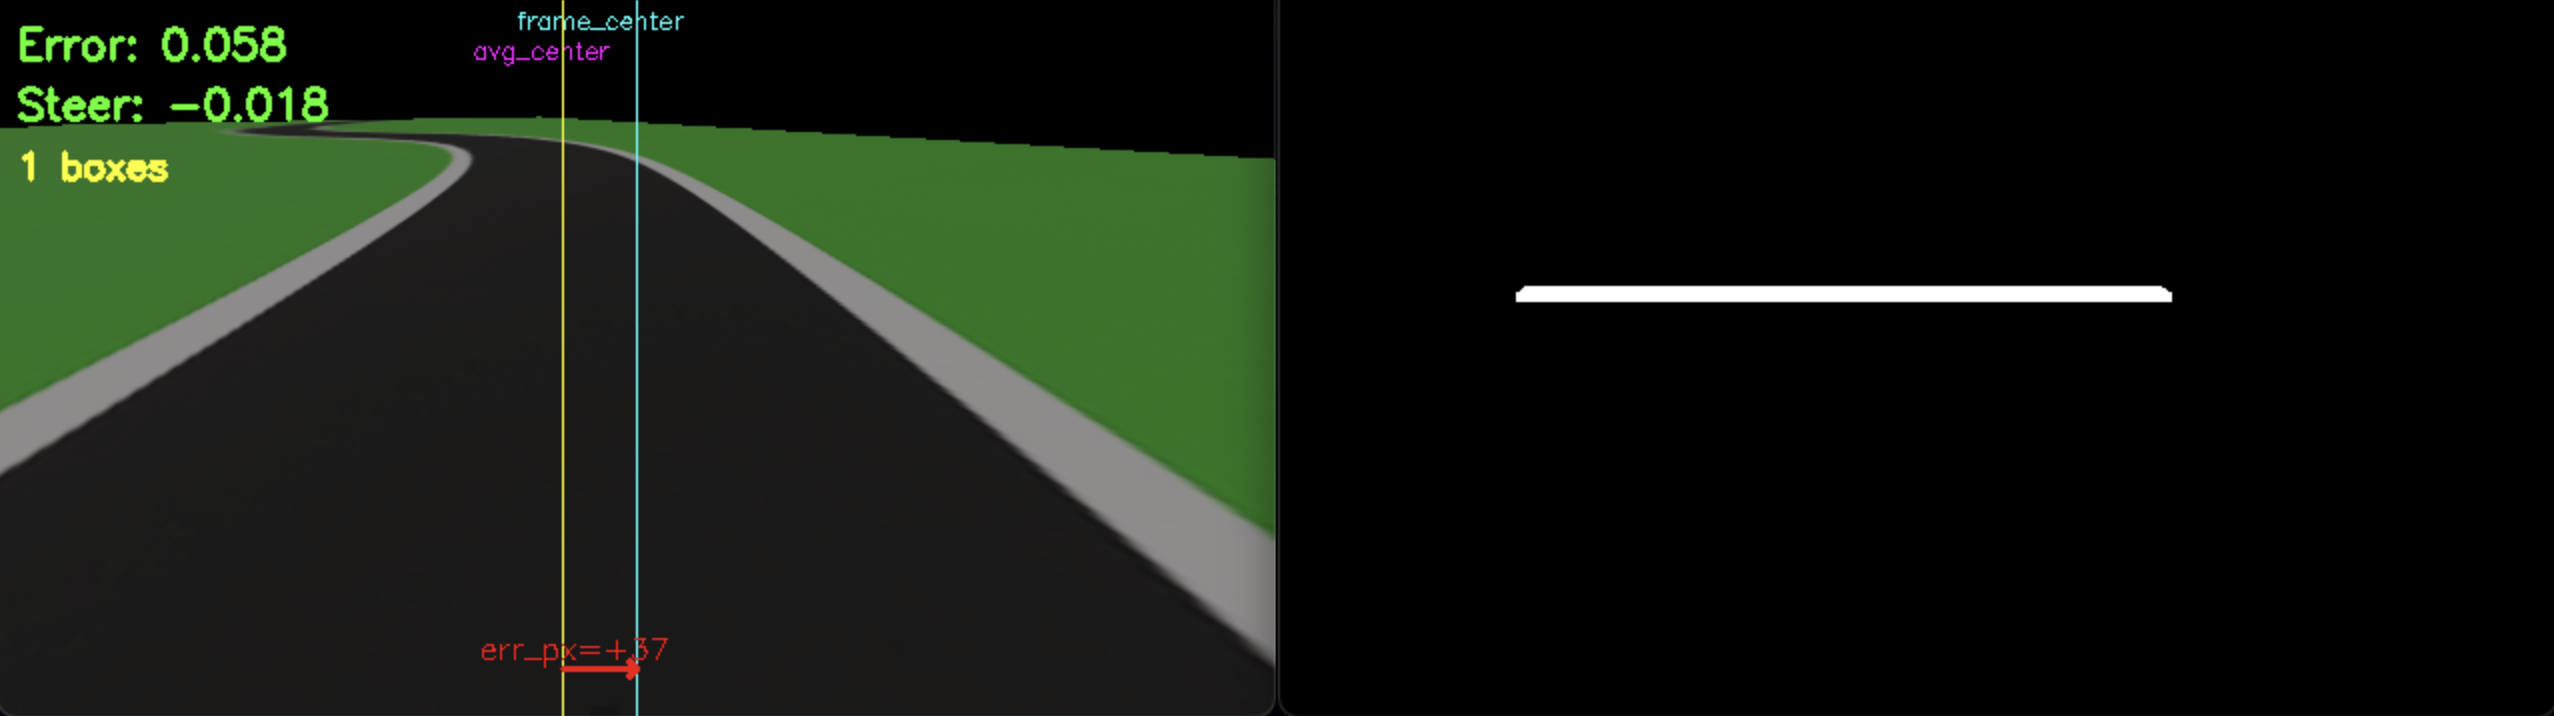
\includegraphics[width=1.0\textwidth]{figures/Fallback_snapshot.png}
  \caption{Fallback-Strategie.}
  \label{fig:fallback}
\end{figure}

Das System definiert eine trapezförmige ROI (ca.\ 40\% Bildhöhe, 2\% Breite) zur 
Fokussierung auf den erwarteten Fahrbahnbereich. Innerhalb dieser ROI erfolgt HSV-basierte Farbsegmentierung für 
dunkelgraue Straßenbereiche und weiße Markierungen, gefolgt von morphologischen Operationen zur Rauschreduktion. 
Die größte erkannte Kontur wird als Straßenbereich interpretiert:




\begin{lstlisting}[style=python,caption={Fallback-Fehlerberechnung},label={lst:fallback_error_calculation}]
  mask_road = cv2.inRange(hsv, road_lower, road_upper)      # Graue Strasse filtern
  mask_white = cv2.inRange(hsv, white_lower, white_upper)   # Weisse Markierungen filtern
  mask0 = cv2.bitwise_or(mask_road, mask_white)
  mask0 = cv2.morphologyEx(mask0, cv2.MORPH_CLOSE, kernel)
  mask0 = cv2.morphologyEx(mask0, cv2.MORPH_OPEN, kernel)
  contours, _ = cv2.findContours(mask0, cv2.RETR_LIST, cv2.CHAIN_APPROX_SIMPLE)
  if contours:
      largest_contour = max(contours, key=cv2.contourArea)
      x, y, w, h = cv2.boundingRect(largest_contour)
      center_x = int(x + w / 2)
      error = (x_set - center_x) / float(max(1, width))   # Fehler normiert an Bildbreite
      mask = np.zeros((height, width), dtype=np.uint8)
      cv2.drawContours(mask, [largest_contour], -1, 255, -1)
      ...  # (Berechnung der Maskenabdeckung)
      self._store_valid_values(error, mask, self.vision_mask_coverage)
      return error, mask

\end{lstlisting}

Der Algorithmus ermittelt die größte Kontur als Straßenbereich und berechnet deren Mittelpunkt. Die normierte 
Differenz zur Bildmitte ergibt den lateralen Fehler, analog zur YOLO-Methode. Bei Erkennungsverlusten greift 
die gleiche Decay-Logik wie in der YOLO-Strategie.

\textbf{Limitierungen:} Die Fallback-Strategie ist anfälliger für variierende Lichtverhältnisse und 
unkonventionelle Straßenbeläge, da sie auf feste Farbschwellenwerte angewiesen ist.
Trotz geringerer Präzision gewährleistet sie grundlegende Spurhaltung 
als Notfallmodus bei YOLO-Ausfall und ist besonders gut für vordefinierte Simulationswege geeignet.



